\documentclass{beamer}
\usepackage[spanish]{babel}
\usepackage[utf8]{inputenc}
\usepackage{graphicx}

\newcommand{\LAl}{{\lambda}}
\newcommand{\NA}{{$\mathbb{N}$}}

\newcommand{\LA}{{$\lambda$}}
\newcommand{\PHI}{{$\varphi$}}

\title[TE]{Distribución de Poisson}
\author[Alba,Dácil,Desireé]{Alba Tomé Rodríguez\\Dácil Batista García\\Desireé Praena Pacheco}
\institute[ULL]{Universidad de La Laguna}
\date[24-04-2014]{24 de abril de 2014}

\usetheme{Madrid}

\definecolor{MiVioleta}{RGB}{122,59,122}
\definecolor{MiAzul}{RGB}{0,88,147}
\definecolor{MiGris}{RGB}{56,61,66}
\setbeamercolor{palette primary}{use=structure,fg=white,bg=MiVioleta}
\setbeamercolor{palette secundary}{use=structure,fg=white,bg=MiAzul}
\setbeamercolor{palette tertiary}{use=structure,fg=white,bg=MiGris}

\begin{document}
\begin{frame}
\titlepage{}
\end{frame}
%%%%%%%%%%%%%%%%%%%%%%%%%%%%%%%%%%%%%%%%%%%%%%%%%%%%%%%%%%%%%%%%%%%%%%%%%%%%%%%%%%%%%%%
\begin{frame}
\frametitle{Indice}
\tableofcontents[pausesections]
\end{frame}
%%%%%%%%%%%%%%%%%%%%%%%%%%%%%%%%%%%%%%%%%%%%%%%%%%%%%%%%%%%%%%%%%%%%%%%%%%%%%%%%%%%%%%%
\section{Introducción}
\begin{frame}
\frametitle{Introducción}
La Poisson es una de las distribuciones de variable discreta más importantes pues los valores que puede tomar son números naturales. Es muy útil cuando la muestra o segmento $n$ es grande y la probabilidad de éxitos $p$ es pequeña. La distribución de Poisson se utiliza en situaciones donde los sucesos son impredecibles o de ocurrencia aleatoria.
\end{frame}
%%%%%%%%%%%%%%%%%%%%%%%%%%%%%%%%%%%%%%%%%%%%%%%%%%%%%%%%%%%%%%%%%%%%%%%%%%%%%%%%%%%%%%%
\section{Historia de la Distribución de Poisson}
\begin{frame}
\frametitle{Historia de la Distribución de Poisson}

\begin{itemize}
\item Fue introducida por primera vez por Simeón Denis Poisson, físico y matemático francés al que se le conoce por sus diferentes trabajos en el campo de la electricidad, la geometría diferencial y la teoría de probabilidades.\pause

\centerline{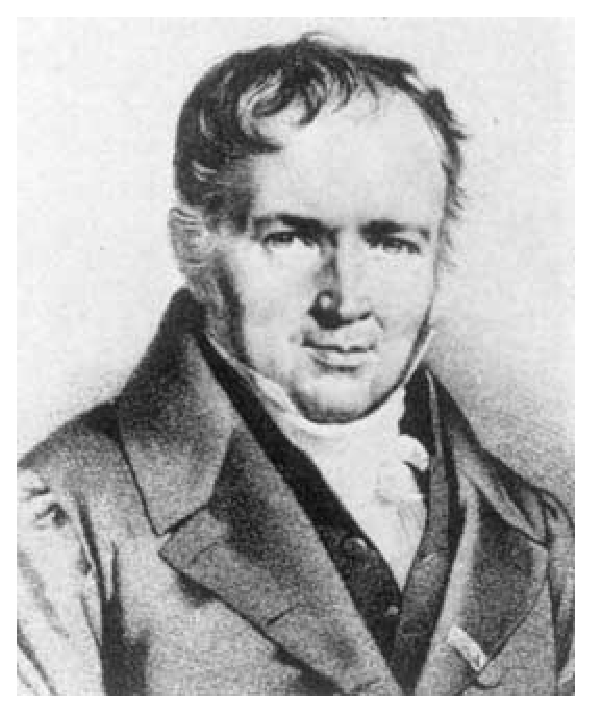
\includegraphics[width=0.25\textwidth]{Poisson.eps}}
\end{itemize}
\end{frame}
%%%%%%%%%%%%%%%%%%%%%%%%%%%%%%%%%%%%%%%%%%%%%%%%%%%%%%%%%%%%%%%%%%%%%%%%%%%%%%%%%%%%%%%%
\begin{frame}
\frametitle{Historia de la Distribución de Poisson}
\begin{itemize}
\item Fue publicada en 1837, junto con su teoría de la probabilidad, donde describe esta última como un acontecimiento fortuito ocurrido en un tiempo o intervalo de espacio bajo las condiciones de que la probabilidad de un acontecimiento ocurra es muy pequeña, pero el número de intentos es muy grande y por tanto el evento ocurre algunas veces.\pause
\item Una aplicación práctica de esta distribución fue hecha por Ladislao Bortkiewicz en 1898 cuando se le dio la tarea de investigar el número de soldados en el ejército prusiano matados accidentalmente por tiro de caballos.
\end{itemize}
\end{frame}

%%%%%%%%%%%%%%%%%%%%%%%%%%%%%%%%%%%%%%%%%%%%%%%%%%%%%%%%%%%%%%%%%%%%%%%%%%%%%%%%%%%%%%%
\section{Conceptos fundamentales}
\begin{frame}
\frametitle{Algunos datos que deberíamos saber}

\begin{itemize}
\item \textbf{Variable aleatoria:} es una aplicación, que a cada valor del espacio muestral le hace corresponder un número real. Se clasifican en:
\pause
\begin{itemize}
\item \textbf{Discretas:} si los números asociados a los sucesos son puntos aislados. Por ejemplo: ''Lanzar una moneda 3 veces y que salga cara''. Los posibles resultados son (0,1,2,3).
\item \textbf{Continuas:} los valores asignados pueden ser cualesquiera dentro de ciertos intervalos. Por ejemplo: ''Tomando la variable nivel de agua de un embalse'', pueden obtenerse valores entre $0$ y $\infty$.
\end{itemize}
\end{itemize}

\end {frame}
%%%%%%%%%%%%%%%%%%%%%%%%%%%%%%%%%%%%%%%%%%%%%%%%%%%%%%%%%%%%%%%%%%%%%%%%%%%%%%%%%%%%%%%%
\subsection{Definición: Distribución de Poisson}
\begin{frame}
\frametitle{Definición: Distribución de Poisson}
Sea $X$ una variable aleatoria de una distribución discreta definida sobre un espacio de probabilidad, se dice que $X$ tiene una distribución de Poisson de parámetro \LA si su función de densidad es:
\begin{block}{Distribución de Poisson}
\centerline{$f(x)=\left\{
	\begin{array}{ll}
        P[X=x]=e^{- \LAl}\frac{\LAl^{x}}{x!} & \mathrm{,si\ } x \in \mathbb{N} \\  
        0 & \mathrm{,en\ otro\ caso\ } 
        \end{array}
\right.$}
\end{block}
donde \LA \ es un parámetro característico de la distribución. A dicha distribución se denomina $P$(\LA).

\end{frame}
%%%%%%%%%%%%%%%%%%%%%%%%%%%%%%%%%%%%%%%%%%%%%%%%%%%%%%%%%%%%%%%%%%%%%%%%%%%%%%%%%%%%%%%
\subsection {Aproximación de la binomial a la Poisson}
\begin{frame}
\frametitle{Aproximación de la binomial a la Poisson}

La Poisson se puede obtener a partir de la binomial.\\
Sea $x$ una variable aleatoria con distribución binomial $B(n,p)$, cuya función de densidad es:
%\begin{block}{Función de densidad}
\centerline{$f(x)={n\choose k}p^k(1-p)^{n-k}$} 
%\end{block}
Cuando el número de pruebas $n \rightarrow \infty$ y la probabilidad del suceso tiende a cero y $np \rightarrow$ \LA \ entonces:

%\begin{block}
\centerline{$\displaystyle\lim f(x)=e^{-\LAl}\frac{\LAl^{k}}{k!}$} 
%\end{block}

que es la función de distribución de Poisson, es decir,\\
%\begin{block}
\centerline{$B(n,p)\rightarrow P$(\LA)} 
%end{block}
bajo las condiciones anteriores.
\end{frame}
%%%%%%%%%%%%%%%%%%%%%%%%%%%%%%%%%%%%%%%%%%%%%%%%%%%%%%%%%%%%%%%%%%%%%%%%%%%%%%%%%%%%%%

\subsection{Función característica}
\begin{frame}
\frametitle{Función característica}
\begin{block}{Función característica}
La función característica viene dada por

\centerline {\PHI \ $ = e^{\LAl(e^{it}-1)}$}
\end{block}

\end{frame}



%%%%%%%%%%%%%%%%%%%%%%%%%%%%%%%%%%%%%%%%%%%%%%%%%%%%%%%%%%%%%%%%%%%%%%%%%%%%%%%%%%%%%%%

\section{Propiedades}
\begin{frame}
\frametitle{Propiedades}
\begin{itemize}
\item \textbf{\large Esperanza}\\
La media o esperanza matemática de $P$(\LA) es:
\centerline {$E(X)=$\LA}
\item \textbf{\large Varianza}\\
Respecto a la varianza,
\centerline {$Var(X)=\LAl=E(X)$}
\item \textbf{\large El parámetro \LA}
El parámetro \LA \ de una distribución de Poisson caracteriza a la misma:
\centerline {\LA \ $ = \displaystyle\lim{np}$}
\end{itemize}
\end{frame}
%%%%%%%%%%%%%%%%%%%%%%%%%%%%%%%%%%%%%%%%%%%%%%%%%%%%%%%%%%%%%%%%%%%%%%%%%%%%%%%%%%%%%%%%
\begin{frame}
\frametitle{Propiedades}
\LA \ se puede obtener de varias formas:
\begin{itemize}
\item $n$ y $p$ conocidas
\centerline {\LA \ $ = np$}
\item A partir de la esperanza
\centerline {\LA \ $ = E(X)$}
\item Estimando a partir de una muestra
\centerline {\LA \ $ = m( X_1,\dots,X_s) = \frac{1}{s}\displaystyle\sum_{i=1}^s X_i$} 
\item A partir de la probabilidad del suceso [$X=0$] ya que
\centerline {$P[X=0] = f(0) = e^{-\LAl}\frac{\LAl^{0}}{0!} = e^{-\LAl}$}
luego \LA \ $ = -\ln P[X=0]$
\end{itemize}
\end{frame}
%%%%%%%%%%%%%%%%%%%%%%%%%%%%%%%%%%%%%%%%%%%%%%%%%%%%%%%%%%%%%%%%%%%%%%%%%%%%%%%%%%%%%%%%
\section{Aplicaciones}
\begin{frame}
\frametitle{Aplicaciones}
\begin{itemize}
\item El número de coches que pasan a través de un cierto punto en una ruta durante un periodo de tiempo.\pause
\item Un número de errores de ortografía que uno comete al escribir una página.\pause
\item Número de llamadas recibidas en una central telefónica por minuto.\pause
\item Distribución de los aminoácidos en las proteínas.\pause
\item Contaje del número de glóbulos rojos en una muestra de sangre.\pause
\item El número de fallos por metro cuadrado de tela.\pause
\end{itemize}
\end{frame}
%%%%%%%%%%%%%%%%%%%%%%%%%%%%%%%%%%%%%%%%%%%%%%%%%%%%%%%%%%%%%%%%%%%%%%%%%%%%%%%%%%%%%%%%
\section{Procedimiento experimental}
\begin{frame}
\frametitle{Procedimiento experimental}
El experimento realizado consiste en aproximar la distribución de los aminoácidos en las proteínas mediante la Poisson.
Un estudio realizado por Gamow revela que es la aproximación a los datos reales observados más acertada con respecto a hipótesis anteriores.\\
Se observaron dipéptidos que podían formarse tomando aminoácidos vecinos, obteniéndose un total de 177. \\
El abanico de probabilidades sería $20x20 = 400$, por tanto en la distribucion de Poisson nuestro \LA \ sería \LA \ $ = \frac {177}{400}=0.442$\\
Para cada $n$ (número de dipéptidos), se tendría lo siguiente:
\centerline {P(n)= e^{- 0.442}\frac{0.442^{n}}{n!}}


\end{frame}


%%%%%%%%%%%%%%%%%%%%%%%%%%%%%%%%%%%%%%%%%%%%%%%%%%%%%%%%%%%%%%%%%%%%%%%%%%%%%%%%%%%%%%%%
\subsection{Resultados. Tablas}
\begin{frame}
\frametitle{Resultados del experimento. Tablas}

Antes de que Gamow asociase el experimento con la distribución de Poisson, se había intentado buscar algun modelo que se adaptase a los resultados. Ejemplos de los obtenidos son el 'Código Diamante' o el 'Código triángulo'. Las siguientes tablas muestra cómo, efectivamente, la Poisson se aproxima con más determinación a los resultados reales observados:

\end{frame}
%%%%%%%%%%%%%%%%%%%%%%%%%%%%%%%%%%%%%%%%%%%%%%%%%%%%%%%%%%%%%%%%%%%%%%%%%%%%%%%%%%%%%%%%
\begin{frame}

\begin{center}
\begin{tabular}{llll}
N dipeptidos & Frec. observada & P(x) (Poisson) & Frec Total 400xP(x) \\
\hline
0 & 264 & 0.6424283410 & 256.9713363872\\
1 & 102 & 0.2842745409 & 113.7098163514\\
2 & 27 & 0.0628957422 & 25.1582968677\\
3 & 4 & 0.0092771220 & 3.7108487880\\
4 & 2 & 0.0010262816 & 0.4105126472\\
5 & 0 & 0.0000908259 & 0.0363303693\\
6 & 0 & 0.0000066984 & 0.0026793647

\end{tabular}
\\
\\
\begin{tabular}{llll}
N dipeptidos & Frec. observada & Codigo Triangulo & Codigo Diamante\\
\hline
0 & 264 & 276 & 305\\
1 & 102 & 86 & 55\\
2 & 27 & 26 & 23\\
3 & 4 & 9 & 7\\
4 & 2 & 3 & 3\\
5 & 0 & 0 & 3\\
6 & 0 & 0 & 2
\end{tabular}
\end{center}
\caption{Comparacion}
\label{tabla}


\end{frame}
%%%%%%%%%%%%%%%%%%%%%%%%%%%%%%%%%%%%%%%%%%%%%%%%%%%%%%%%%%%%%%%%%%%%%%%%%%%%%%%%%%%%%%%%
\subsection{Resultados. Gráficos}
\begin{frame}
\frametitle{Resultados del experimento. Gráficos}


\begin{figure}[!ht]{Comparacion Poisson-Diamante-Triangulo\\}
\centering
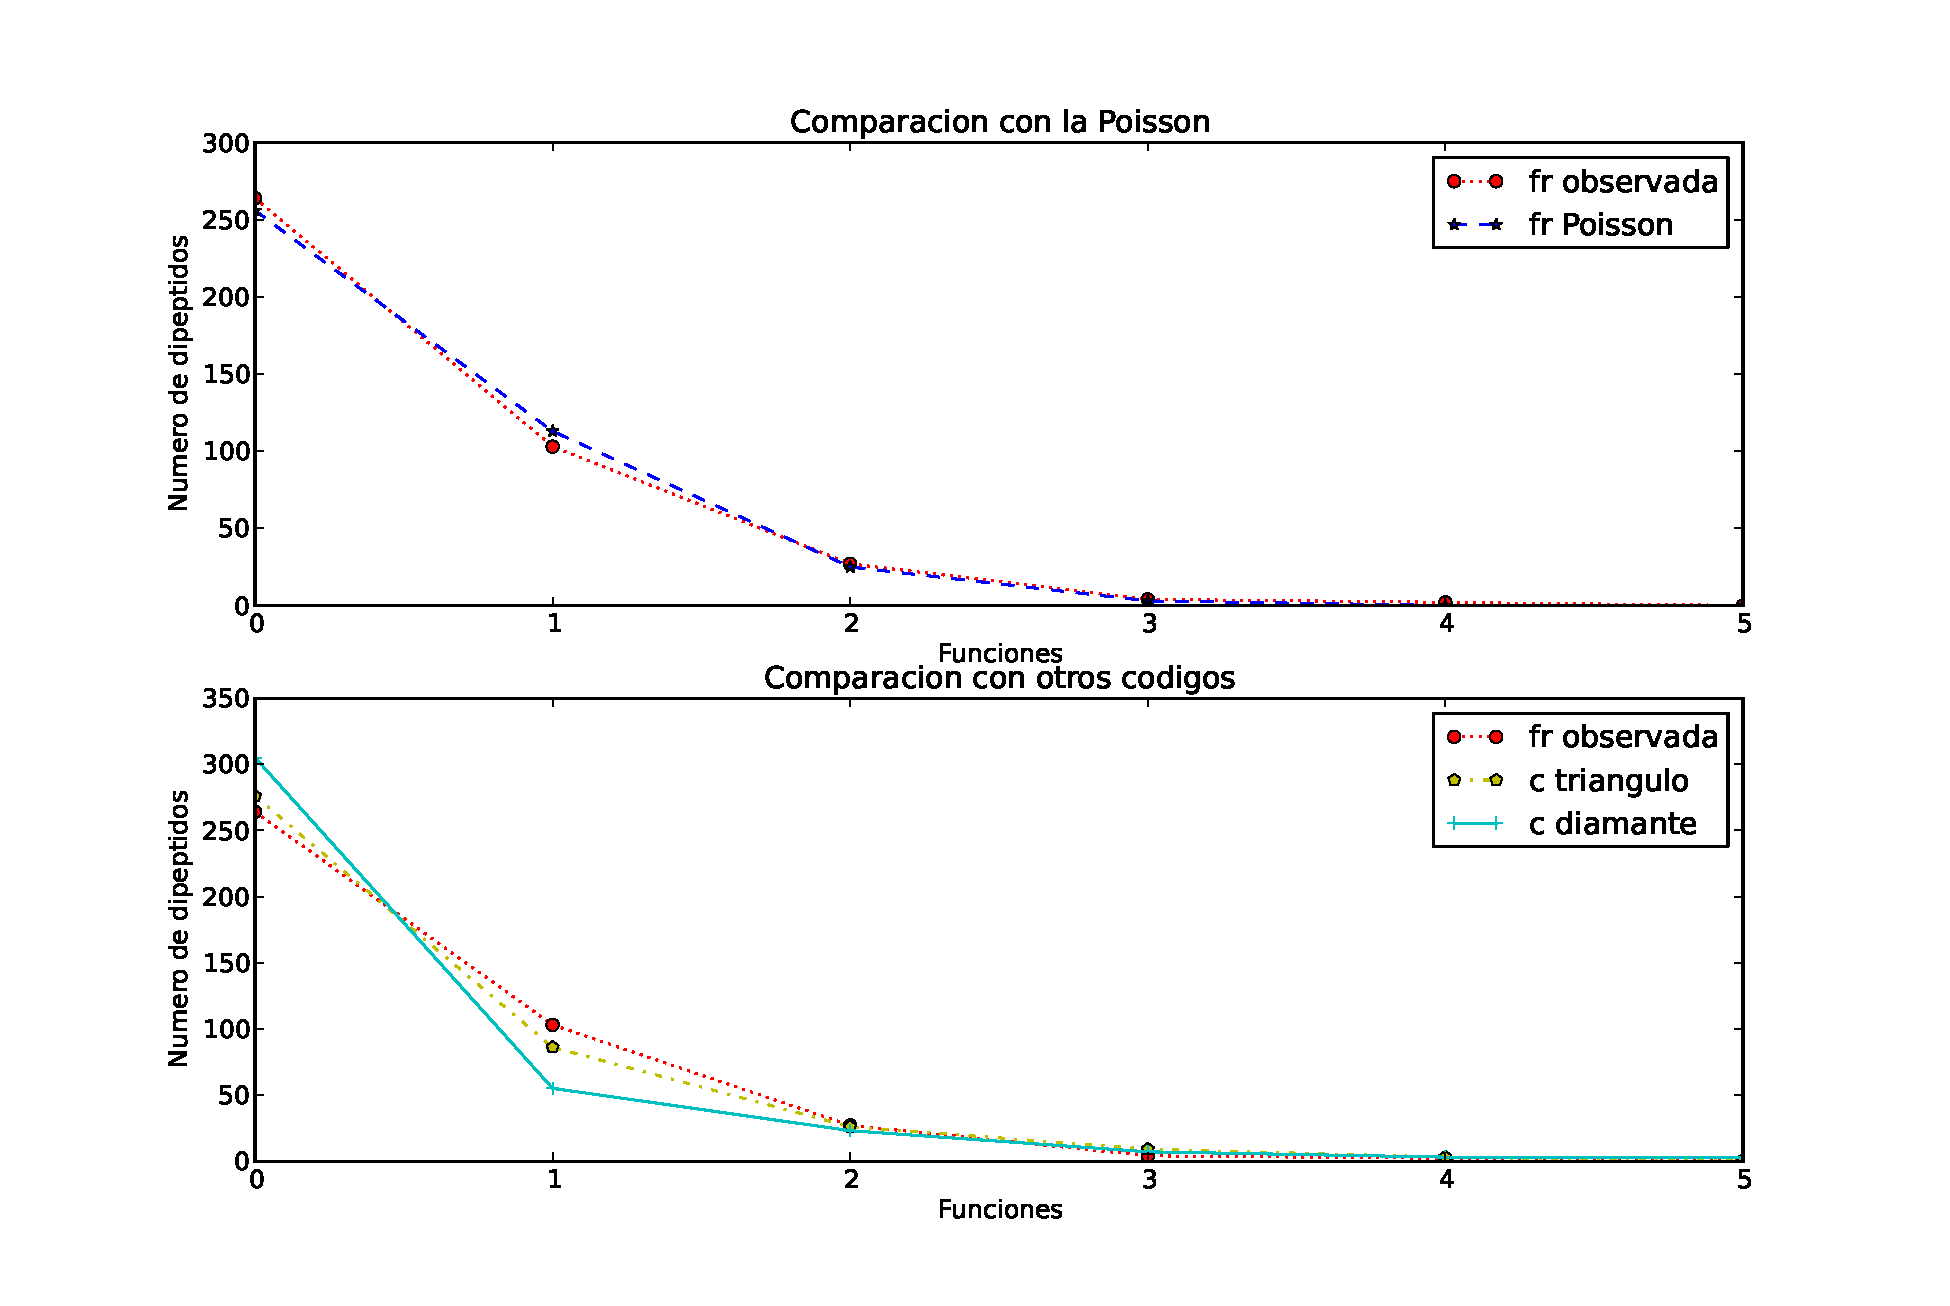
\includegraphics[width=0.7\textwidth]{comparacion.eps}
\caption{Comparacion}
\end{figure}

\end{frame}
%%%%%%%%%%%%%%%%%%%%%%%%%%%%%%%%%%%%%%%%%%%%%%%%%%%%%%%%%%%%%%%%%%%%%%%%%%%%%%%%%%%%%%%%%%%%
\section{Bibliografía}
\begin{frame}
\frametitle{Bibliografía}
\begin{thebibliography}{10}
\beamertemplatebookbibitems
\bibitem{}
Fundamentos de Probabilidad en Estadística. G.Alonso, J.Ocaña, C.M.Cuadras.
\bibitem{}
Estadística Teórica y Aplicada. Andrés Nortes Checa.
\bibitem{}
www.itch.edu.mx/academic/industrial/sabaticorita/private/05Distr
\bibitem{}
www.aulafacil.com/CursoEstadistica/Lecc-29-est.htm
\end{thebibliography}
\end{frame}





%%%%%%%%%%%%%%%%%%%%%%%%%%%%%%%%%%%%%%%%%%%%%%%%%%%%%%%%%%%%%%%%%%%%%%%%%%%%%%%%%%%%%%%%%%%%%




\end{document}

